\documentclass[fontset=ubuntu]{ctexart}

% \usepackage{ctex}
\usepackage{graphicx} % 图片
\usepackage{subfigure} %子图片
\usepackage{minted} % 代码
\usepackage{listings} % 代码
\usepackage{enumerate} % 有序列表
\usepackage{float} % 设置位置
\usepackage{hyperref} % 网页链接
\usepackage{fancyhdr} % 页眉页脚

\title{\Huge \textbf{实验报告三 \\ 命令行环境\&Python}}
\author{\textit{潘奕霖}}
\date{https://github.com/PLY1024/system-develop-tools\\ \today}
\pagestyle{fancy}

\fancyhead{}
\fancyhead[R]{\textsl{\leftmark}}
\fancyfoot{}
\fancyfoot[L]{https://github.com/PLY1024/system-develop-tools}
\fancyfoot[R]{\thepage}
\setlength{\headheight}{14pt}
\addtolength{\topmargin}{-5pt}

\begin{document}

\maketitle
\newpage

\tableofcontents
\newpage

\section{命令行环境学习感悟}
有了之前使用shell的基础,命令行环境的有关命令也不是那么抽象。目前感知最强,最有用的可能就是tmux,通过键盘就能操作,极大提升效率,还能做到断开会话连接但保持程序运行,经过自定义后能有很好的体验。远程连接在未来很重要,但对于没有服务器的我们来说,在本地虚拟机上实现ssh连接的操作还是有点复杂。至于进程控制,可能在安装或者编译的时候会有大用,能暂停任务,改变输出界面的位置,甚至在断开shell连接之后还能运行程序,还是很强大的。

\section{命令行环境知识点}
\subsection{中止某个正在进行的进程}
输入Ctrl-c会使shell向进程发送SIGINT信号,SIGINT代表SIGnal INTerrupt,用于中止进程。输入Ctrl+\verb|\|也可以中止进程,其发送的是SIGQUIT信号。进程有处理以上两个信号的能力,因此在接受信号后可能不会中止,而SIGKILL信号是进程无法处理的,在收到信号后一定会中止。

\subsection{一个不会被SIGINT信号中止的Python程序}
以下是一个能处理SIGINT信号的Python程序,在收到SIGINT信号后会输出
I got a SIGINT, but I am not stopping,这时可以输入Ctrl+\verb|\|来中止这个程序,或者使用\mintinline{shell}|kill -TERM <PID>|来中止这个程序。
\begin{figure}[htb]
    \centering
    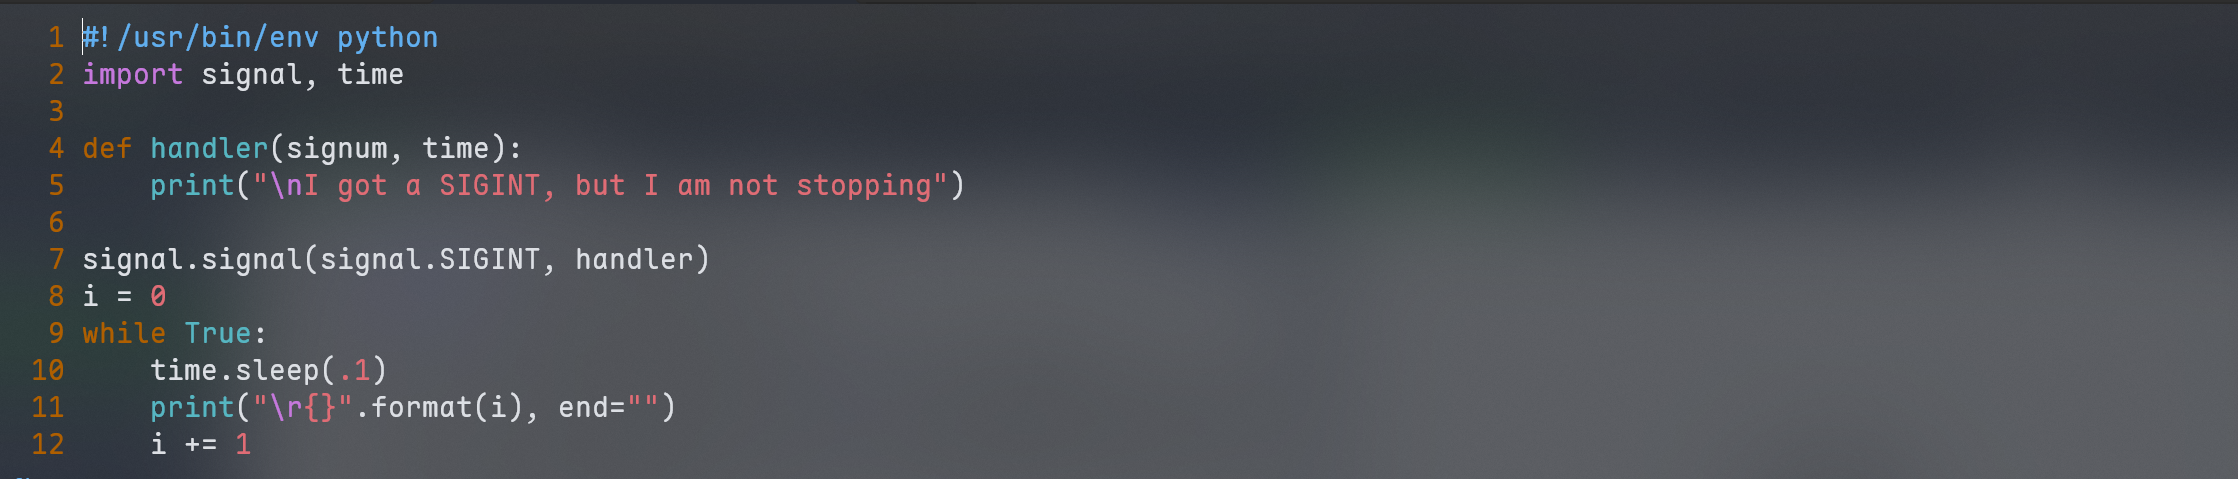
\includegraphics[width=0.75\linewidth]{Sigint_1.png}
    \caption{程序截图}
    \label{fig:Sigint_1}
\end{figure}

\begin{figure}[htb]
    \centering
    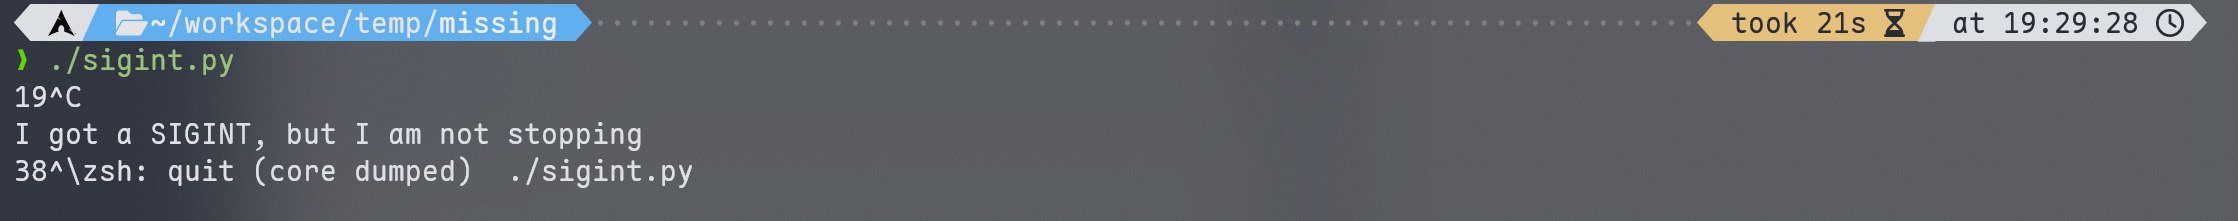
\includegraphics[width=0.75\linewidth]{Ctrl_1.png}
    \caption{输出效果}
    \label{fig:Ctrl_1}
\end{figure}

\subsection{进程暂停与恢复}
输入Ctrl-Z会向进程发送SIGSTOP信号使其暂停,使用\mintinline{shell}|fg|和\mintinline{shell}|bg|分别能使其在前台或后台恢复运行。可以使用\mintinline{shell}|jobs|列出当前未完成的进程以及它们的任务序号,并通过\%来引用任务序号,对进程进行操作。要使一个进程在开始时就在后台运行,需要在命令最后加上\&。而一个已经在运行的进程需要先暂停后再使用\mintinline{shell}|bg|恢复后台运行。

使用\mintinline{shell}|nohup|在开始进程时指定其不会被SIGHUP中止,即避免其在关闭终端时停止,对于一个已经在运行的进程,使用\mintinline{shell}|disown|来避免其被终端关闭。

\mintinline{shell}|kill|可以用于发送各种信号,包括中止信号,暂停信号。

\subsection{设定别名}
在shell的配置文件,如.bashrc,.zshrc中添加别名设置语句就可以为命令添加别名,提高使用效率。设置语句的格式为:\mintinline{shell}|alias <别名>="命令"|,如\mintinline{shell}|alias ll="ls -lh"|。效果如下,注意要\mintinline{shell}|source ~/.zshrc|以使修改生效。
\begin{figure}[htb]
    \centering
    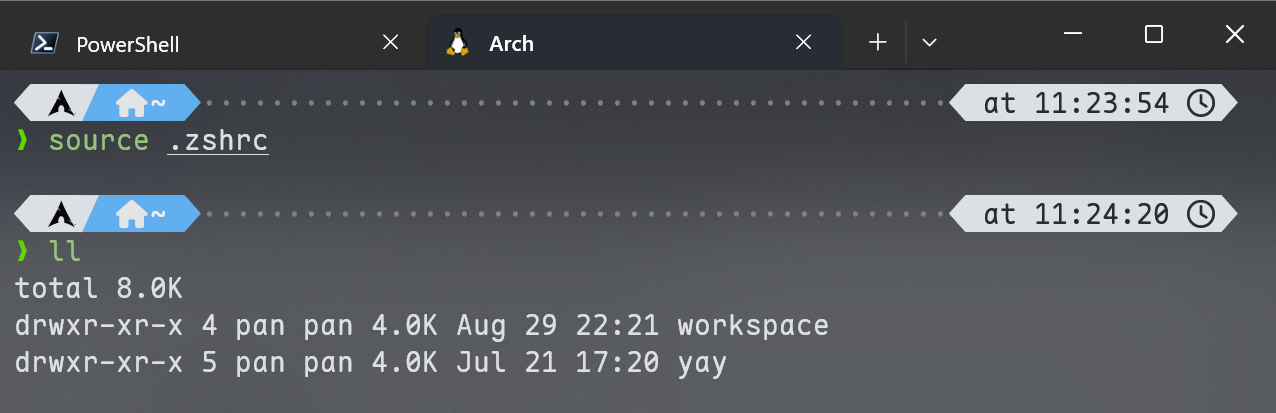
\includegraphics[width=0.75\linewidth]{alias_1.png}
    \caption{设置别名}
    \label{fig:alias_1}
\end{figure}

\subsection{任务控制}
使用\mintinline{shell}|pgrep|查找pid并使用\mintinline{shell}|pkill|结束进程。\mintinline{shell}|pgrep|能根据进程关键字搜寻pid,\mintinline{shell}|pkill|的-f参数能搜索进程名。
\begin{figure}[htb]
    \centering
    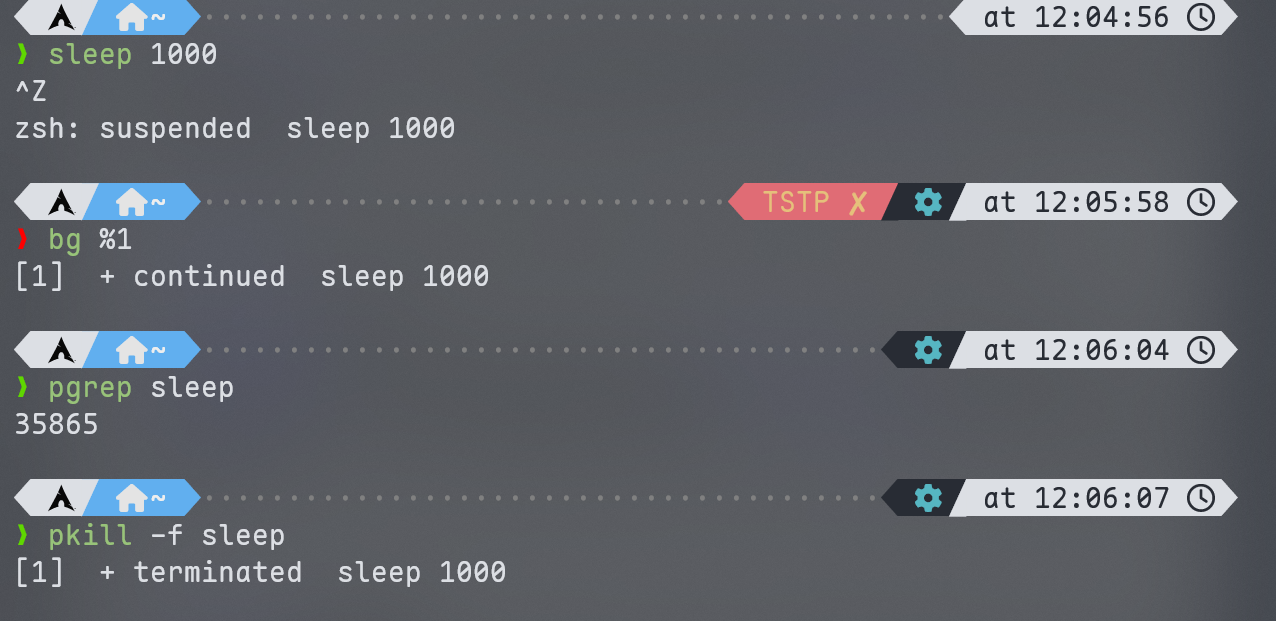
\includegraphics[width=0.75\linewidth]{pkill_1.png}
    \caption{通过搜索进程名结束进程}
    \label{fig:pkill_1}
\end{figure}

\subsection{顺序执行进程}
需要在某个进程结束后进行另一个进程,可以使用\mintinline{shell}|wait|,在进程结束后再执行下一条命令。但\mintinline{shell}|wait|命令只能对子进程使用,可以使用如下的函数实现在不同的shell中顺序执行进程。
\begin{figure}[htb]
    \centering
    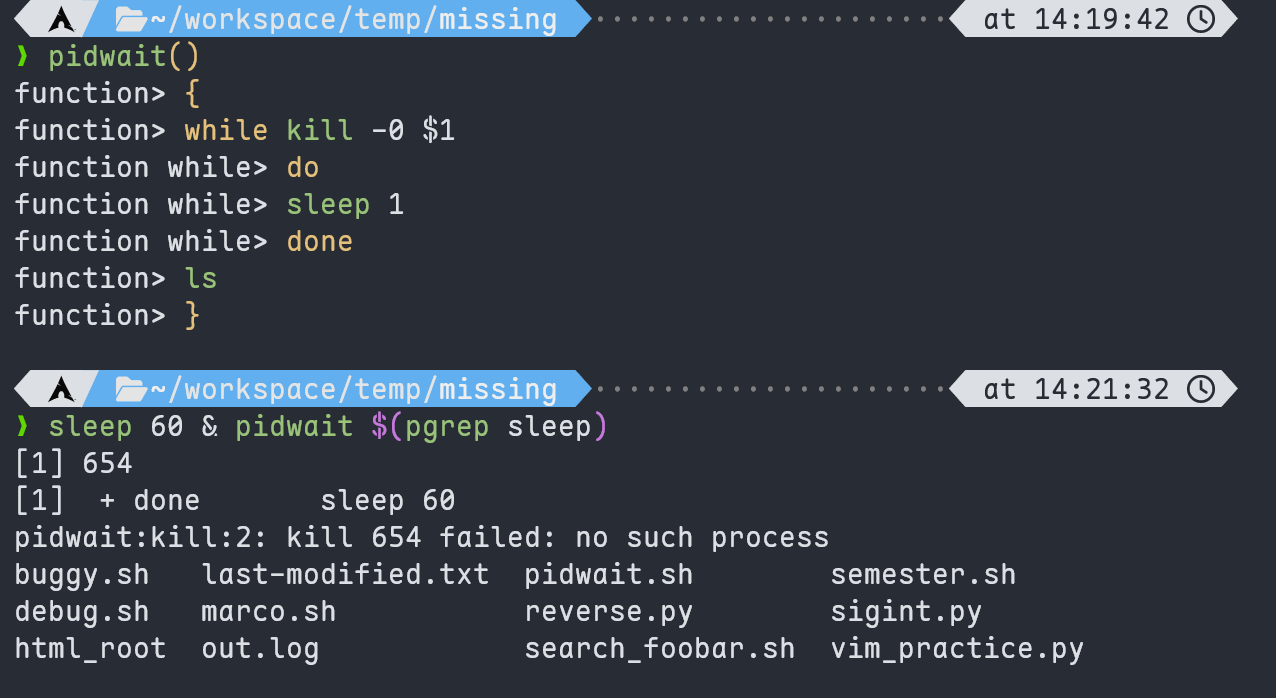
\includegraphics[width=0.75\linewidth]{pidwait_1.png}
    \caption{pidwait函数}
    \label{fig:pidwait_1}
\end{figure}

shell中while 判断的是命令的返回值是否为0,不为0则跳出循环,\mintinline{shell}|kill -0|在进程存在时会返回0,在进程不存在时会返回非0的状态码。在当做参数传入的进程结束时,会跳出while循环,执行\mintinline{shell}|ls|操作。

\subsection{终端复用}
tmux是一个终端复用工具,能开启多个会话,每个会话可以有多个窗口,每个窗口能被分割为多个面板。tmux界面的最下方会列出当前的窗口和一些信息。使用\mintinline{shell}|prefix c|能开启新的窗口,通过\mintinline{shell}|prefix p|,\mintinline{shell}|prefix n|能在不同的窗口间切换。使用\mintinline{shell}|prefix "|能将当前面板水平分为上下两部分,\mintinline{shell}|prefix|加空格可以切换面板的排布,\mintinline{shell}|prefix|加方向键能在不同的面板间切换。

\mintinline{shell}|prefix x|关闭当前面板,\mintinline{shell}|Ctrl-d|退出当前的窗口,
\mintinline{shell}|prefix d|中断与当前会话的连接,在远程连接时有用。\mintinline{shell}|tmux ls|能列出当前的会话,用于重新连接和关闭会话。

以下是我自定义后的tmux,且修改prefix为Ctrl-a。
\begin{figure}[htb]
    \centering
    \includegraphics[width=0.75\linewidth]{tmux_1.png}
    \caption{自定义效果}
    \label{fig:tmux_1}
\end{figure}

\begin{figure}[htb]
    \centering
    \includegraphics[width=0.75\linewidth]{tmux_2.png}
    \caption{配置文件}
    \label{fig:tmux_2}
\end{figure}

\subsection{储存配置文件}
创建一个存放配置文件的git仓库,将配置文件移到此处并通过软链接链接至home文件夹。这样在修改配置文件时能避免因为错误的配置导致无法复原,且能将一处的修改同步到各个设备上,在使用新设备时也能快速进行配置。配置的方法也很简单,只需要运行一个能为文件创建软链接的shell脚本,再去安装所需要的插件即可。
\begin{figure}[htb]
    \centering
    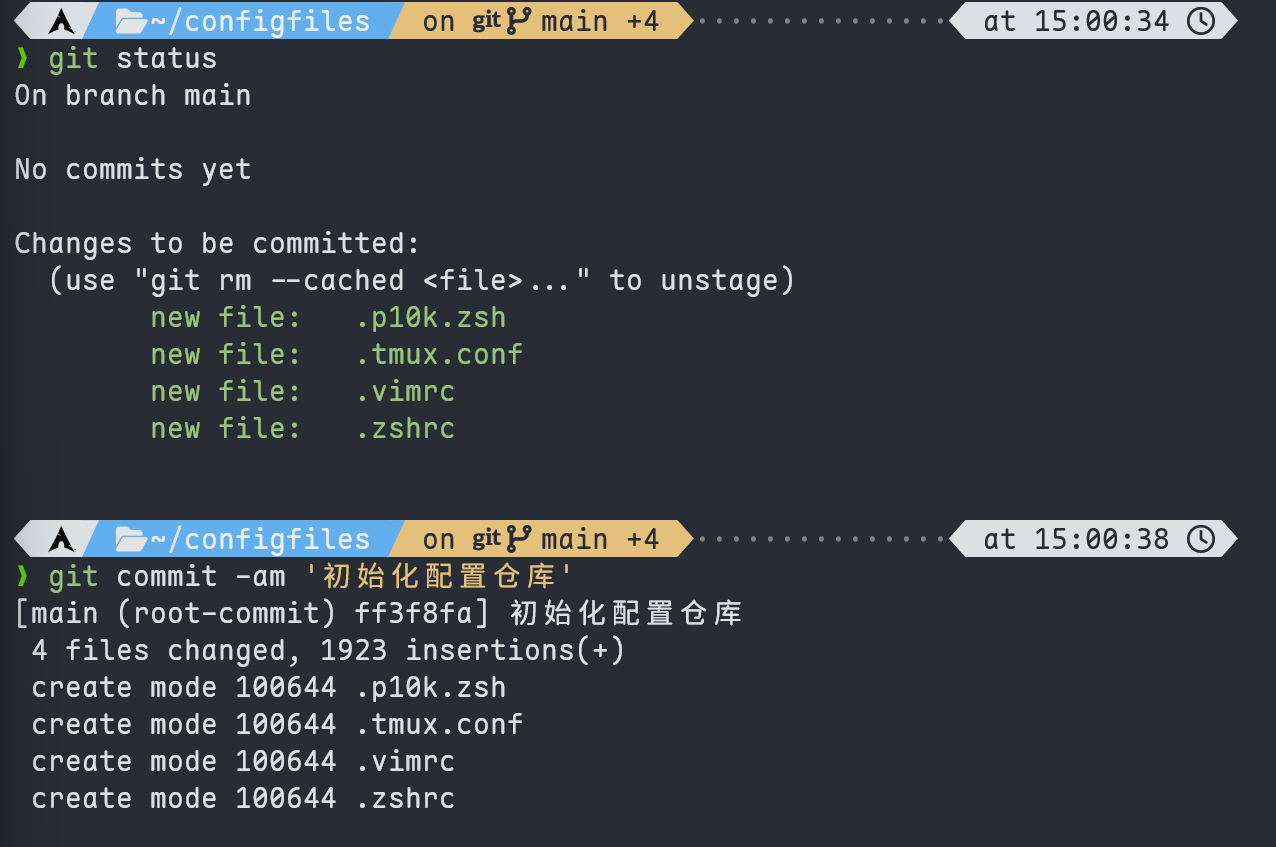
\includegraphics[width=0.75\linewidth]{config_1.png}
    \caption{创建仓库}
    \label{fig:config_1}
\end{figure}

\begin{figure}[htb]
    \centering
    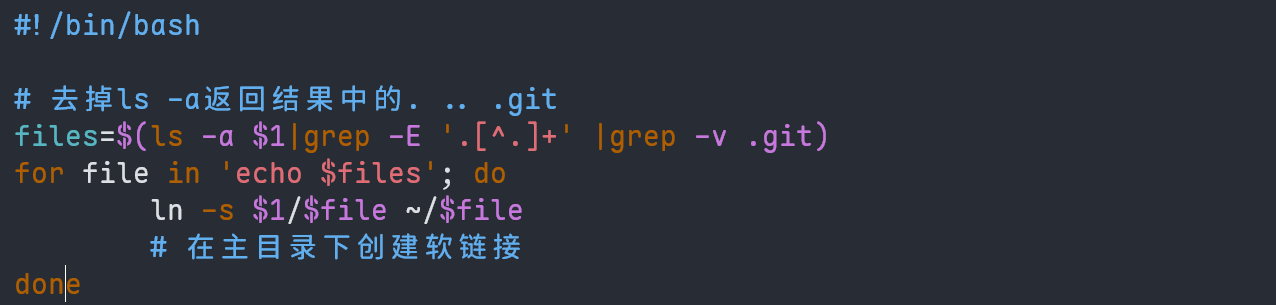
\includegraphics[width=0.75\linewidth]{config_2.png}
    \caption{配置脚本}
    \label{fig:config_2}
\end{figure}

\subsection{远程连接}
使用\mintinline{shell}|ssh <username>@<service>|以登录服务器,服务器可以通过URL指定,也可以通过IP指定。

使用\mintinline{shell}|ssh-keygen|命令生成密钥,储存在\mintinline{shell}|/.ssh|文件夹内。密钥可以避免每次输入都输入密码,提高效率,也可以为密钥设置密码,提高安全性。
\begin{figure}[htb]
    \centering
    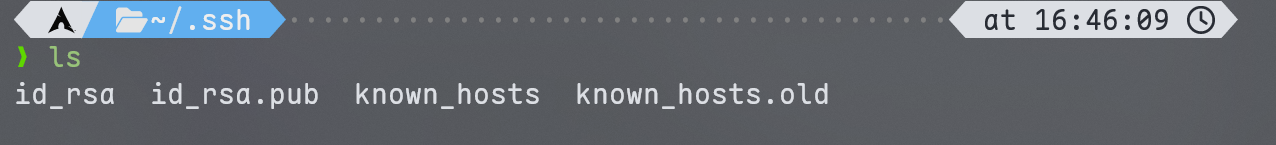
\includegraphics[width=0.75\linewidth]{ssh_1.png}
    \caption{密钥文件}
    \label{fig:ssh_1}
\end{figure}

\subsection{使用PowerShell连接wsl中的虚拟机}
这看起来是一件非常无聊的事情。首先需要修改虚拟机的ssh配置文件,\verb|sudo vim /etc/ssh/sshd_config|打开配置文件,设定端口为2222,监听地址为0.0.0.0,修改\verb|PermitRootLogin yes|与\verb|PasswordAuthentication yes|。之后再运行\mintinline{shell}|sudo systemctl status sshd|,查看ssh的状态,如果为inactive,需要\mintinline{shell}|sudo systemctl restart sshd|重新启动ssh。然后就可以再PowerShell内使用\mintinline{shell}|ssh root@localhost -p 2222|连接wsl了。

\section{Python学习感悟}
相对于C,Python是非常容易上手的,不用管头文件,不用关mian函数,直接就可以开写。而且Python没有C那样抽象的声明和定义分开的情况,对变量的初始化赋值也不用考虑先声明变量的类型,定义函数也不用管返回值的问题。最让我感到高兴的是Python的函数在\mintinline{Python}|return|多个值时会自动返回一个元组,让能返回的信息大大增加,而解压赋值这个操作的存在能让我轻松获取返回值。

Python的文件操作也十分简单,按行读取内容时只要使用\mintinline{Python}|for|就可以,还有\mintinline{Python}|with|语句帮助打开文件,为文件赋予别名,在操作完成后帮助我们关闭文件。各种模块更是让Python变得即强大又易用。

不过要注意的是Python虽然方便,在安装时要注意环境变量的设置,在编写代码时还要注意缩进的内容,不要混用tab和空格。

\section{Python知识点}
\subsection{输入输出}
使用\mintinline{Python}|input|输入,输入的值为字符串,可以顺带输出提示信息。\mintinline{Python}|print|进行输出,可以输出各种格式,还可以\mintinline{Python}|end=|指定输出的结尾。
如以下的语句在输出结束后不会换行:
\mint{Python}|print("hello", end="")|

\subsection{格式化输出}
Python支持三种格式化输出字符串的形式,分别是\%s,format和f。

\%s即对应位置输出,\mintinline{Python}|"Name is %(name)s and age is %(age)s"|,需在字符串后通过\%连接一个字典\mintinline{Python}|% {"name": "Mike", "age": 8}|,通过键取得字典中的值,填入字符串。

format支持索引填值和键填值,字符串使用format方法为其传值。
\mint{Python}|"Name is {0} {0} and age is {1}".format("Mike", 8)|
\mint{Python}|"Name is {name} and age is {age}".format(name="Mike", age=8)|

f则可以直接将命名空间内的变量值填入字符串。
\begin{listing}[htb]
    \begin{minted}{Python}
    name = input("Your name: ")
    age = input("Your age: ")
    result_4 = f"My name is {name}, my age is {age}"
    \end{minted}
\end{listing}

\subsection{特殊的运算符}
Python中有一些特殊的运算符和一些特殊的运算语句,提供了多样的用法。
\begin{itemize}
    \item 幂运算:\mintinline{Python}|**|能直接实现幂运算,而C还要调用函数
    \item 交换赋值:\mintinline{Python}|x, y = y, x|直接就能交换x与y的值
    \item 与或非:不同于C,Python中逻辑运算使用\mintinline{shell}|and or not|三个运算符
    \item 属于:\mintinline{Python}|in|运算符用于判断前者是否是后者的一部分,且对Python内置类型都适用
    \item 是:\mintinline{Python}|is|能够判断两个变量的id值是否相同,即他们所引用的值在内存中的地址是否相同
    \item 集合操作:\& | - \verb|^| 在Python中属于集合操作,分别代表取交集,取并集,取差集,取对称差集,以及大于号小于号用于判断子集关系
\end{itemize}

\subsection{\mintinline{Python}|if|,\mintinline{Python}|while|的特殊点}
不同于C,Python中的条件判断语句使用的是如下语句,用缩进和冒号分隔出不同的代码级别。
\begin{listing}[htb]
    \begin{minted}{Python}
    if a == 1:
        return true
    elif a == 2:
        return false
    else:
        return None
    \end{minted}
\end{listing}

Python的while语句也不同于C,其还有else的分支。当while循环是由于条件语句为false而结束时,会进入else的分支,而当循环是由于break而结束时,不会进入else分支。
\begin{listing}[htb]
    \begin{minted}{Python}
    while flag:
        print('1')
    else:
        print('2')
    \end{minted}
\end{listing}

\subsection{for遍历}
语法为\mintinline{Python}|for A in B|,B为一个可迭代对象,包括列表、字典、字符串、元组、集合,A为变量名,且可以不止一个。要遍历得到数组,可以使用\mintinline{Python}|range|,如\mintinline{Python}|for i in range(0, 8)|可以遍历得到0到7,\mintinline{Python}|range|为一个生成器,第一个参数设置起始值,第二个参数设置终点值且无法取到,第三个参数设置步长。

\subsection{字符串}
Python中的字符串可以用双引号和单引号进行赋值,而不像C++中只能用双引号。Python中的字符串支持加法操作,即拼接字符串,还支持乘法以进行多次拼接。
\begin{figure}[htb]
    \centering
    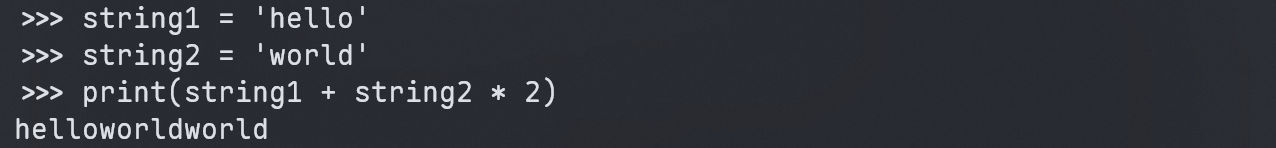
\includegraphics[width=0.75\linewidth]{string_1.png}
    \caption{字符串操作}
    \label{fig:string_1}
\end{figure}

字符串支持索引取值和切片,能快速取得字符串的片段,还内置了许多方法,如\mintinline{Python}|find replace isdigit|等。\mintinline{Python}|find|方法能找到字符串中是否出现了目标字符或字符串。\mintinline{Python}|replace|方法不仅能找到目标字符串,还能将其替换为其他字符串。\mintinline{Python}|isdigit|方法可以检测字符串是否由纯阿拉伯数字组成,这在检测用户输入时非常有用。

注意,在输出特殊字符,如单引号双引号时,同C一样需要加上\verb|\|。

\subsection{字典}
字典是“key:value”的键值对,key是不可变类型且不能重复。使用\mintinline{Python}|dict|创建字典,可以使用for循环对字典进行遍历,取得的是字典的键,使用len方法可以取得字典键的个数。字典可以直接通过对键值对的操作进行取值和赋值,能直接创建键值对,还支持使用update方法用字典来更新字典。

\subsection{定义函数}
使用\mintinline{Python}|def|定义函数,在定义时会检测语法错误,定义时可以不写返回值,即返回\mintinline{Python}|None|。
\begin{listing}[htb]
    \begin{minted}{Python}
    def 函数名(参数列表):
        函数描述
        函数体
        return 数据
    \end{minted}
\end{listing}

Python中的函数没有声明一说,直接定义即可,且不用显式指定返回值。

\subsection{导入模块}
使用\mintinline{Python}|import ...|导入包,包括Python内置的模块,第三方模块和自定义模块。还可以使用\mintinline{Python}|from ... import ...|导入某个模块中的子模块。使用模块名就可以使用模块的功能。导入一个模块中的所有内容使用的命令是\mintinline{Python}|from ... import *|,也可以为模块设置别名,只要在\mintinline{Python}|from|语句后加上\mintinline{Python}|as ...|即可,就能使用别名调用模块。

要注意的是使用\mintinline{Python}|import ...|导入模块后,在使用模块时需要带上模块的全名,比如使用\mintinline{Python}|import os.path|导入了os模块内的path模块,在使用path模块的\mintinline{Python}|split|函数时要以\mintinline{Python}|os.path.split()|的形式使用,不可省去\mintinline{shell}|os.path|。

\subsection{PIL转换图片格式}
用PIL模块打开图像时无需指定图片格式,直接Image.open即可,Image模块会根据图片内容自己确定打开的格式,使用save保存时也无需指定格式,由文件后缀名即可确定保存格式。
\begin{figure}[htb]
    \centering
    \subfigure[代码]{
    \label{fig:convert_1}
    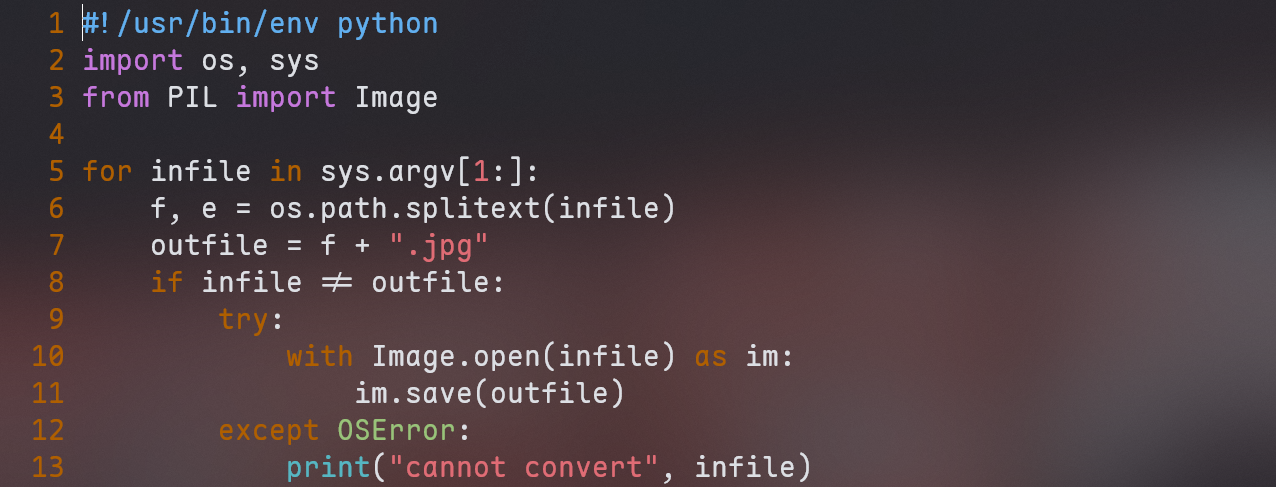
\includegraphics[width=0.45\linewidth]{convert_1.png}
    }\subfigure[创建结果]{
    \label{fig:convert_2}
     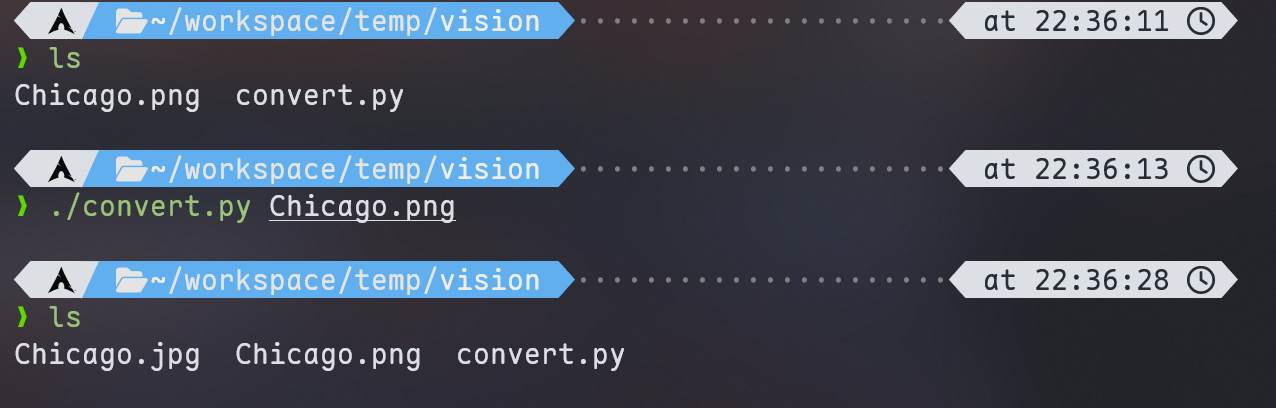
\includegraphics[width=0.45\linewidth]{convert_2.png}
    }
    \caption{转换结果}
    \label{convert_2}
\end{figure}

\subsection{PIL创建略缩图}
以下的代码本应该创建一张图像的缩略图,并通过save指定以JPEG格式保存,但不知为什么指定的格式不生效,缩略图以.thumbnail为拓展名进行了保存。将拓展名修改为JPEG后可以正常看到略缩图,或许需要指定拓展名才能正确保存。
\begin{figure}[htb]
    \centering
    \subfigure[代码]{
    \label{fig:thumbnails_1}
    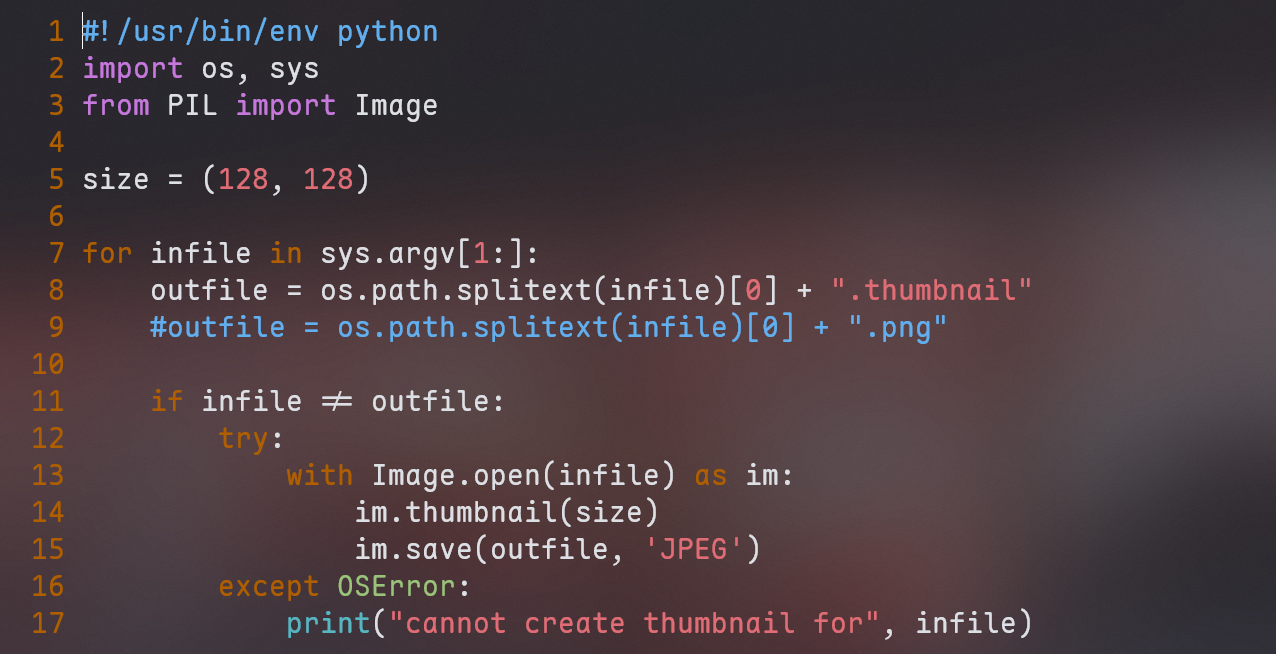
\includegraphics[width=0.45\linewidth]{thumbnails_1.png}
    }\subfigure[创建结果]{
    \label{fig:thumbnails_2}
     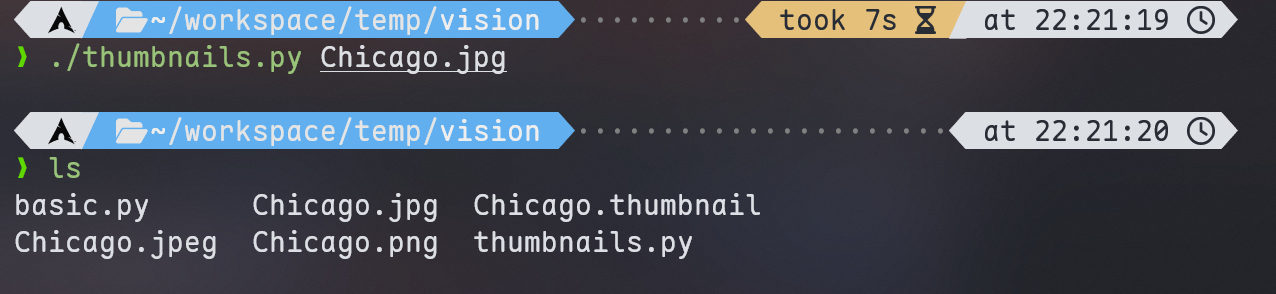
\includegraphics[width=0.45\linewidth]{thumbnails_2.png}
    }
    \caption{创建缩略图}
    \label{thmubnails}
\end{figure}

\begin{figure}[htb]
    \centering
    
\includegraphics[width=0.4\linewidth]{thumbnails_3.png}
    \caption{缩略图}
    \label{fig:thumbnails_3}
\end{figure}

\subsection{PIL图像调整}
resize方法能改变图像大小,只需要指定目标大小。使用rotate方法可以旋转图像对象,能够指定旋转的角度。要注意的是如果想在原图像的基础上修改图像大小和方向,需要对原图像进行赋值,否则只是产生了一个临时的图像对象。

PIL还支持对图像某一部分进行裁切,即使用crop方法,传入的参数是裁切的位置,可以是一个四元组,要注意的是图像的左上角为坐标原点,四元组中四个数字分别对应裁切位置的左,上,右,下。使用paste能进行贴图,参数为要粘贴的图像对象和粘贴的位置,位置参数的设置和corp方法相同。
\begin{figure}[htb]
    \centering
    \subfigure[修改图片]{
    \label{fig:modify_1}
    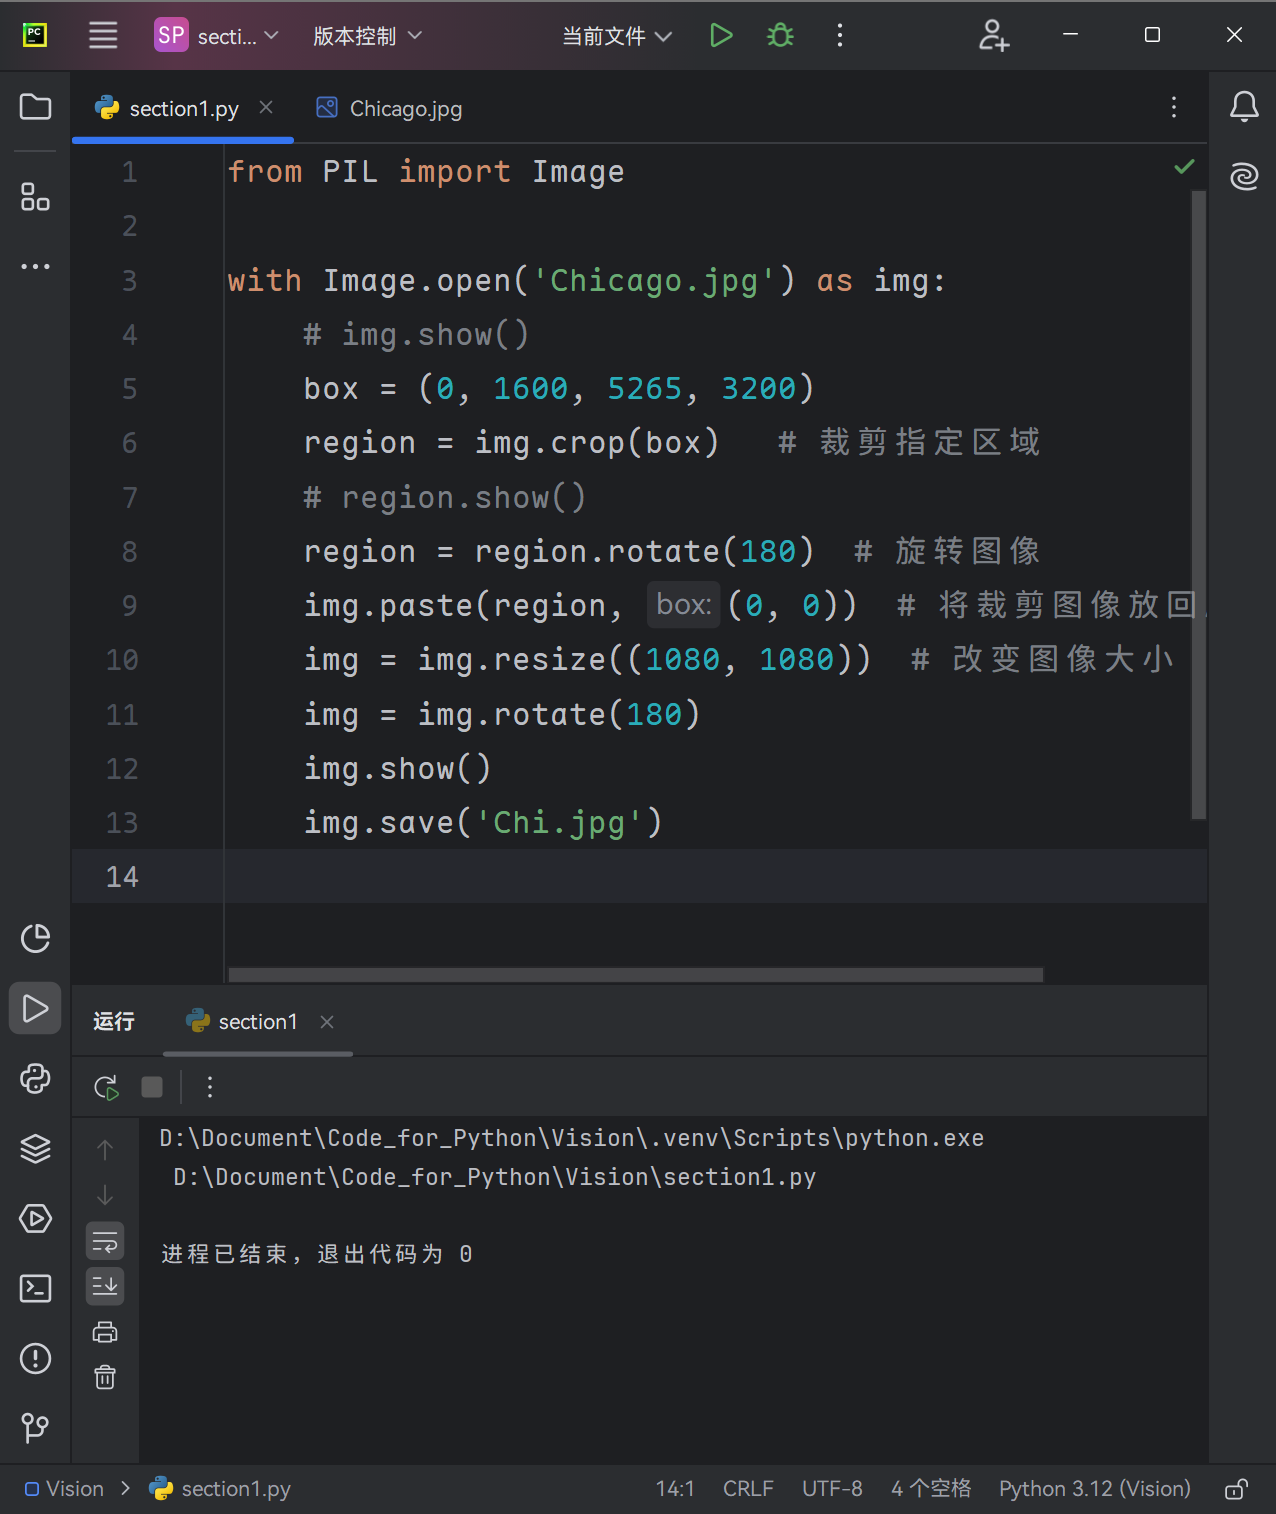
\includegraphics[width=0.45\linewidth]{modify_1.png}
    }\subfigure[修改后的图片]{
    \label{fig:Chi_1}
     
\includegraphics[width=0.45\linewidth]{Chi_1.jpg}
    }
    \caption{调整图像}
    \label{modify}
\end{figure}

\subsection{pylab绘制点与线}
在安装matplotlib包后,可以很方便地使用其内置的pylab模块进行绘图。在使用Image模块读入图片后,可以借助numpy模块的array函数将图片存入数组,再使用pylab模块的imshow函数显示图像,接着就可以绘制点与线。

用两个列表存放点的坐标,注意要坐标数相对应。使用pylab的plot函数就能进行绘图,当传入参数为两个存放坐标的列表时,其会绘制点,当传入为两点对应坐标时,绘制线,可以指定点和线的样式。title函数能设定标题的内容,位置,字体。axis函数控制坐标轴有关的信息。
\begin{figure}[htb]
    \centering
    \subfigure[代码]{
    \label{fig:dot_line_1}
    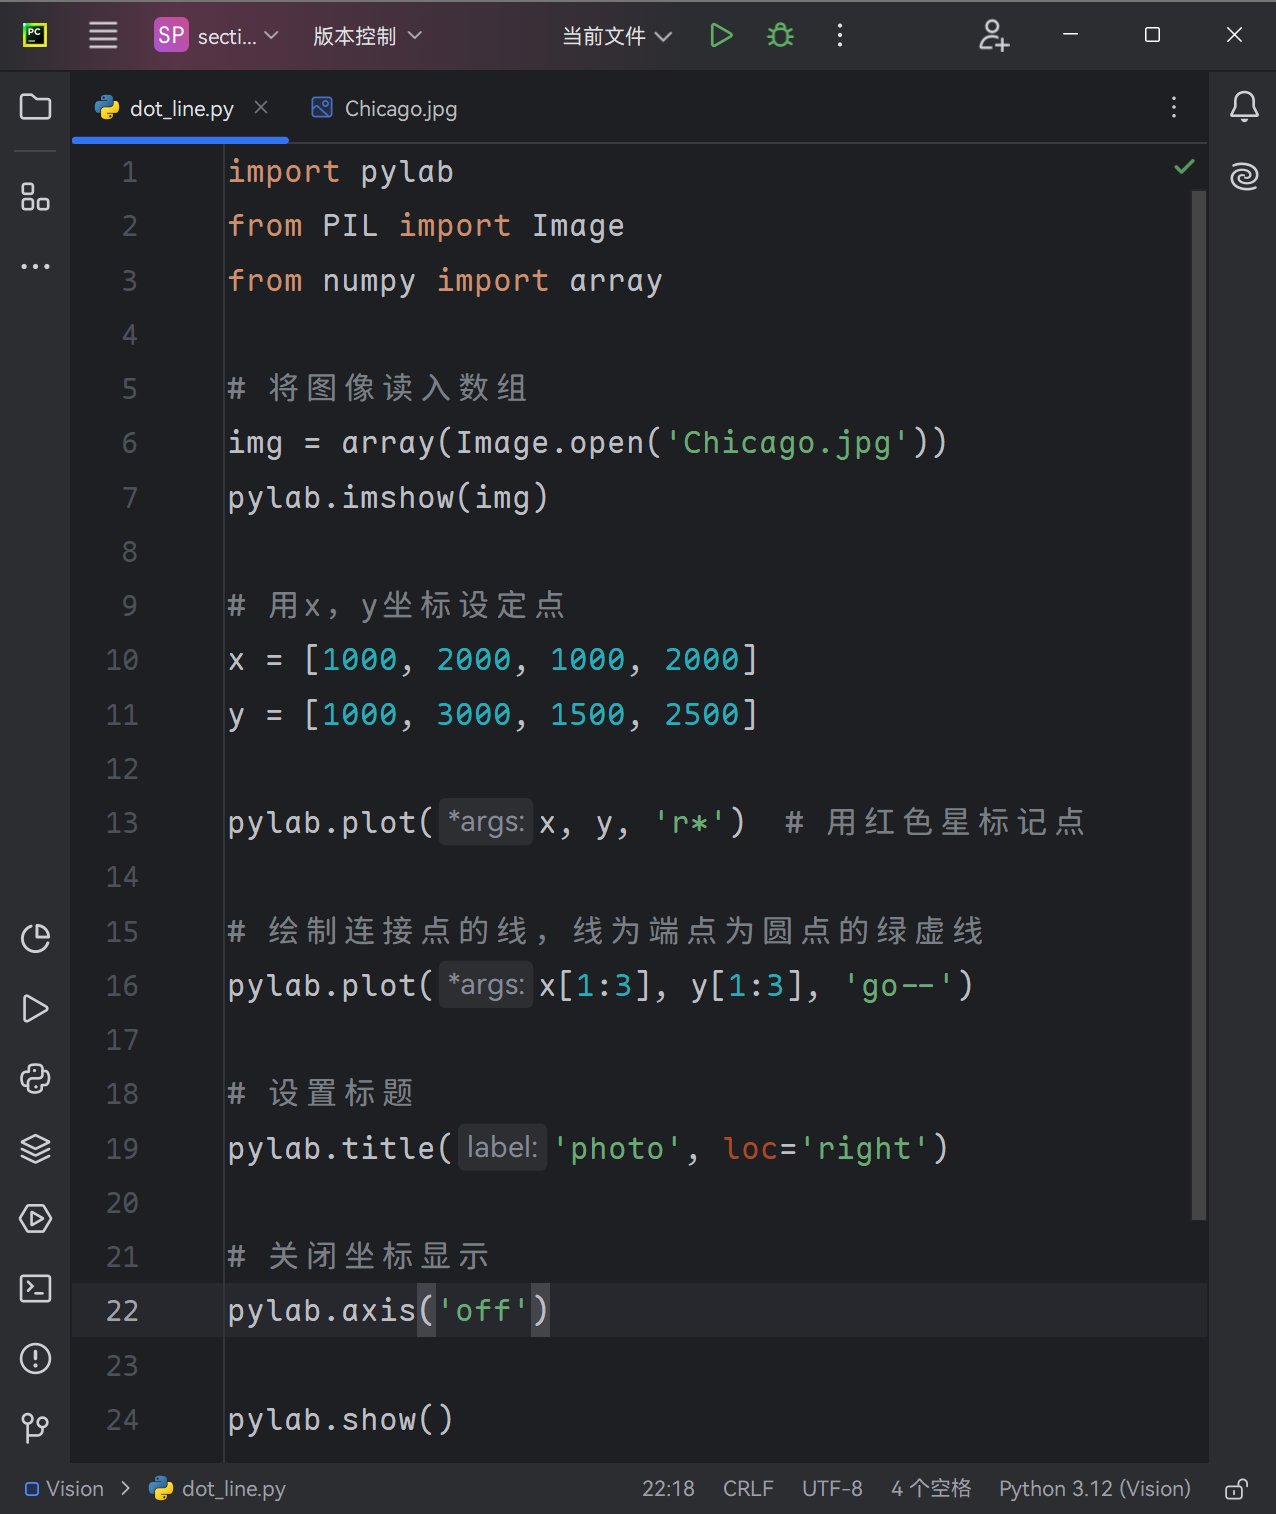
\includegraphics[width=0.45\linewidth]{dot_line_1.png}
    }\subfigure[效果]{
    \label{fig:dot_line_2}
     
\includegraphics[width=0.45\linewidth]{dot_line_2.png}
    }
    \caption{绘制点与线}
    \label{dot_line}
\end{figure}

\subsection{pylab绘制图像轮廓和直方图}
使用counter函数能显示图像的轮廓,使用hist函数能绘制图像的直方图,但由于其只接受一维数组,需要对图像使用flatten函数进行压平处理。
\begin{figure}[htb]
    \centering
    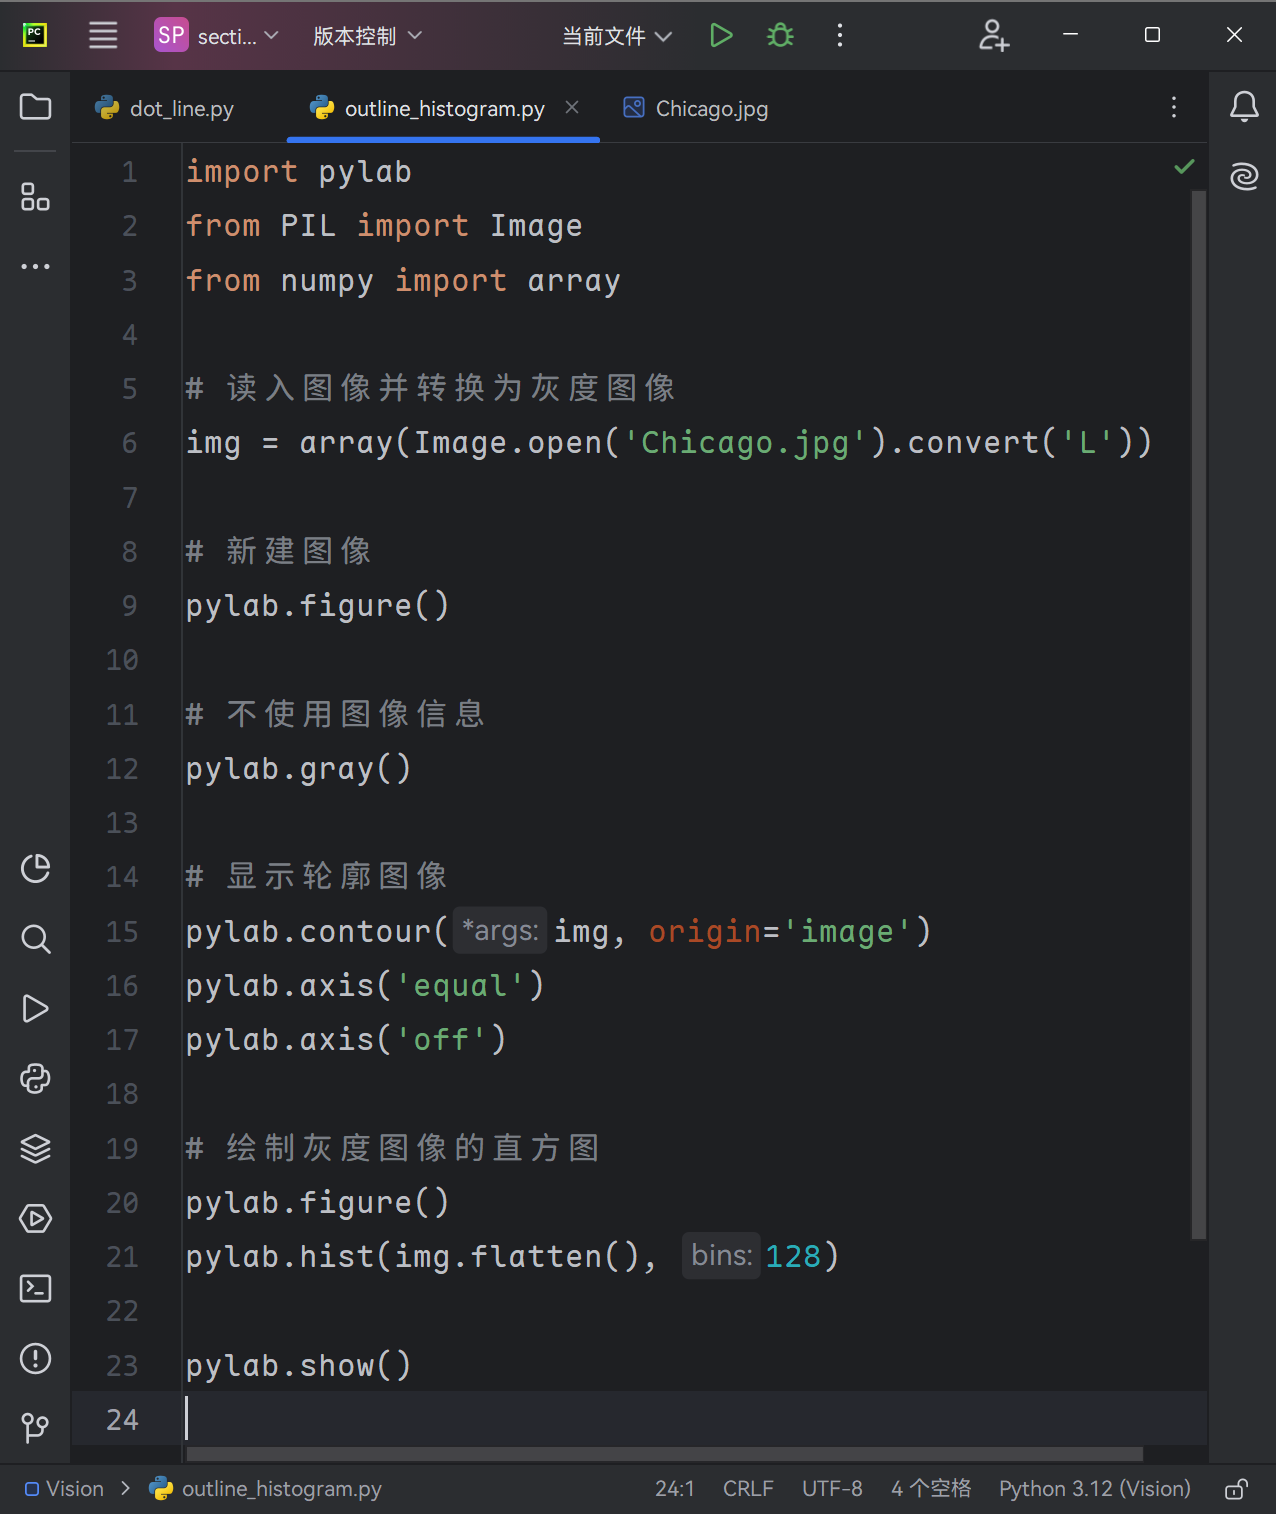
\includegraphics[width=0.4\linewidth]{outline_histogram_1.png}
    \caption{操作代码}
    \label{fig:outline_histogram_1}
\end{figure}

\begin{figure}[htb]
    \centering
    \subfigure[轮廓图]{
    \label{fig:outline_histogram_3}
    
\includegraphics[width=0.45\linewidth]{outline_histogram_3.png}
    }\subfigure[直方图]{
    \label{fig:outline_histogram_2}
     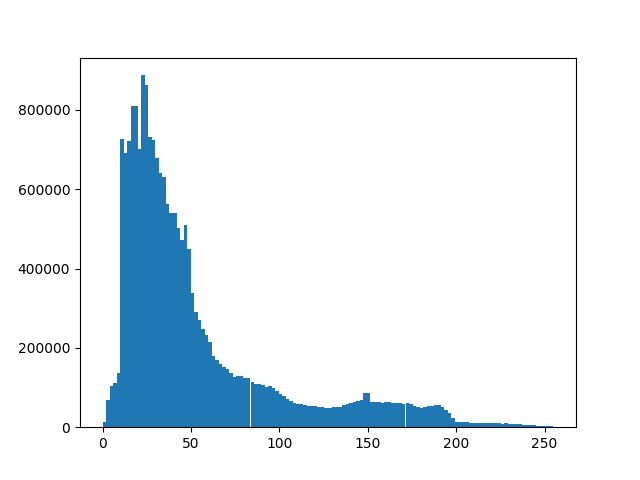
\includegraphics[width=0.45\linewidth]{outline_histogram_2.png}
    }
    \caption{处理结果}
    \label{outline_histogram}
\end{figure}

\subsection{对numpy数组中的图像进行缩放}
numpy的数组对象没有对图像缩放的现成方法,需要借助PIL对图像对象的缩放方式。PIL内Image模块的fromarray函数能将numpy数组对象转换为图像对象,不过需要注意的是数组内存储的数据类型。将图片存入数组时默认以“uint8”类型储存,但也可以指定为其他数据类型,不过在转换回图片对象前需要将数据类型转换为“uint8”类型,即使用\verb|uint8(img)|函数。对“uint8”类型的数组,使用Image模块的fromarray函数就能将其转换回图像对象。一个能对数组中图像进行缩放的函数如下:
\begin{listing}[htb]
    \begin{minted}{Python}
    def imgresize(img,  size):
        pil_img = Image.fromarray(uint8(img))
        return array(pil_img.resize(size)
            
    \end{minted}
\end{listing}

\subsection{使用pickle保存与读取数据}
使用pickle模块的dump和load模块可以很方便的将数据存入.pkl文件与读取,支持几乎所有的Python对象,但也意味着保存的文件只能用Python进行读取。以下的代码对.pkl文件进行保存与读取:
\begin{listing}[htb]
    \begin{minted}{Python}
    with open('file.pkl', 'wb') as f:
        pickle.dump(data, f)

    with open('file.pkl', 'rb') as f:
        data = pickle.load(f)
            
    \end{minted}
\end{listing}

打开文件时要注意模式,\mintinline{Python}|'wb'|即以二进制模式打开,进行写的操作,会清空文件的内容;而\mintinline{Python}|'rb'|以二进制模式打开,进行读取操作。

除了pickle模块外,json模块也提供了序列化的功能,不过其为了维持与其他编程语言的通用性,只支持了其他语言也有的数据类型。

\end{document}